\pdfoutput=1
% \documentclass[red,handout,professionalfont]{beamer}
\documentclass[red,professionalfont]{beamer}
\usepackage{multimedia}
\usepackage{chessboard}
\usepackage{url}
\usepackage{amssymb}  % the check symbol 
\include{pythonlisting}
\usepackage{tikz}
\usepackage{tikz-qtree}
\usetikzlibrary{decorations.pathreplacing,positioning}
%\bibliography{mujstyl}
\theoremstyle{definition}
\newtheorem{definice}{Definition}[section]
\newtheorem{thm}{Theorem}[section]
\newtheorem{idea}{Idea}[section]
\newtheorem{cor}[thm]{Corrollary}
\newtheorem{lem}[thm]{Lemma}
\newtheorem{obs}[thm]{Observation}
\newtheorem{rem}[thm]{Remark}
\newtheorem{ex}[thm]{Example}
\newtheorem{quizz}[thm]{Question}
\newcommand{\pomega}{\mbox{$\mathcal{P}(\omega)$}}
\newcommand{\cont}{\mbox{$\mathfrak c$}}
\newcommand{\ba}{\mbox{${\mathbb B}$}}
\newcommand{\0}{\mbox{${\bf 0}$}}
\newcommand{\F}{\mbox{${\mathcal F}$}}
\newcommand{\rest}{\mbox{$\upharpoonright$}}
\newcommand{\cl}[1]{\mbox{$\overline{#1}$}}
\newcommand{\yes}{\textcolor{green}{$\checkmark$}}
\newcommand{\no}{\textcolor{red}{$\times$}}
\renewcommand{\emph}[1]{{\bf #1}}
\mode<presentation>
{
\useinnertheme{rounded}

\usecolortheme{whale}
\usecolortheme{orchid}

\setbeamerfont{block title}{size={}}

%   \useoutertheme{default}
%   \usetheme{Copenhagen}
%   \useoutertheme{default}
  \setbeamercovered{invisible}
}
\setbeamertemplate{navigation symbols}{} 
\usepackage[utf8]{inputenc}
\usepackage[czech,english]{babel}
\usepackage{lmodern}
%\usepackage{times}
\usepackage[T1]{fontenc}


\tikzset{onslide/.code args={<#1>#2}{%
  \only<#1>{\pgfkeysalso{#2}} % \pgfkeysalso doesn't change the path
}}

\tikzstyle{hilight}=[red,ultra thick]
\tikzstyle{active}=[yellow,ultra thick]
\tikzstyle{memory}=[blue]



\title[]{Znalostní agenti I.\\ (7. přednáška)}

% Dnes se podíváme na jednoduché "goal-based" agenty
% a ukážeme si obecné postupy 


% \author[]{Jonathan L. Verner}
% \institute[Charles University, Prague] % (optional,but mostly needed)
% {
%   Department of Logic\\
  %   Faculty of Philosophy\\
%   Charles University in Prague
% }
\date[]{}
% \subject{}
%\pgfdeclareimage[height=1cm]{university-logo}{UK-logo}
%\logo{\pgfuseimage{university-logo}}

\begin{document}

\AtBeginSection[]
{
  \begin{frame}<beamer>
    \begin{block}{}
%    \begin{centering}
    \hfill\insertsection\hfill\
 %   \end{centering}
    \end{block}
    %\tableofcontents[currentsection]
  \end{frame}
}

\AtBeginSubsection[]
{
  \begin{frame}<beamer>
    \begin{block}{}
  %  \begin{centering}
    \hfill\insertsubsection\hfill\
   % \begin{centering}
    \end{block}
    %\tableofcontents[currentsection]
  \end{frame}
}

%#################################################################

\begin{frame}{} \titlepage
%{\ \hfill \includegraphics[width=1cm]{UK-logo}\hfill\ }
\end{frame}


% 
% \begin{frame}\frametitle{CSP --- NP-úplnost}
% \end{frame}

\begin{frame}\frametitle{Znalostní agenti}
\begin{itemize}
 \item svět je často částečně pozorovatelný\pause
 \item inteligentní agenti se rozhodují na základě dostupných znalostí\pause
 \item inteligentní agenti by si měli umět tyto znalosti rozšiřovat\pause
 \begin{itemize}
   \item pozorováním světa\pause
   \item odvozováním z již získaných znalostí
 \end{itemize}
\end{itemize}
\end{frame}

\begin{frame}\frametitle{Dračí doupě}
\emph{Cíl:} Projít jeskyní, najít poklad.\pause\\
\emph{Překážky:}\pause
\begin{itemize}
 \item zapáchající příšera (\emph{Wumpus}), která sežere každého, kdo jí přijde do cesty.\pause
 \item hluboké jámy, do kterých lze spadnout a hrdina se nedostane ven.
\end{itemize}\pause
\emph{Pravidla:}
\begin{itemize}
 \item v sousedství jámy to fouká\pause
 \item v sousedství příšery to zapáchá\pause
 \item poklad se třpytí
 \item příšera, která umře, vydá skřek slyšitelný po celé jeskyni\pause
 \item je možno jít dopředu nebo se otočit o 90 stupňů\pause
 \item není možno chodit skrz stěny, náraz do zdi pořádně bolí\pause
 \item je možno sebrat poklad\pause
 \item je možno střelit jeden šíp, který letí daným směrem dokud nezabije příšeru nebo nenarazí na stěnu\pause
\end{itemize}
\end{frame}

\begin{frame}\frametitle{Schéma jeskyně}
\begin{center}
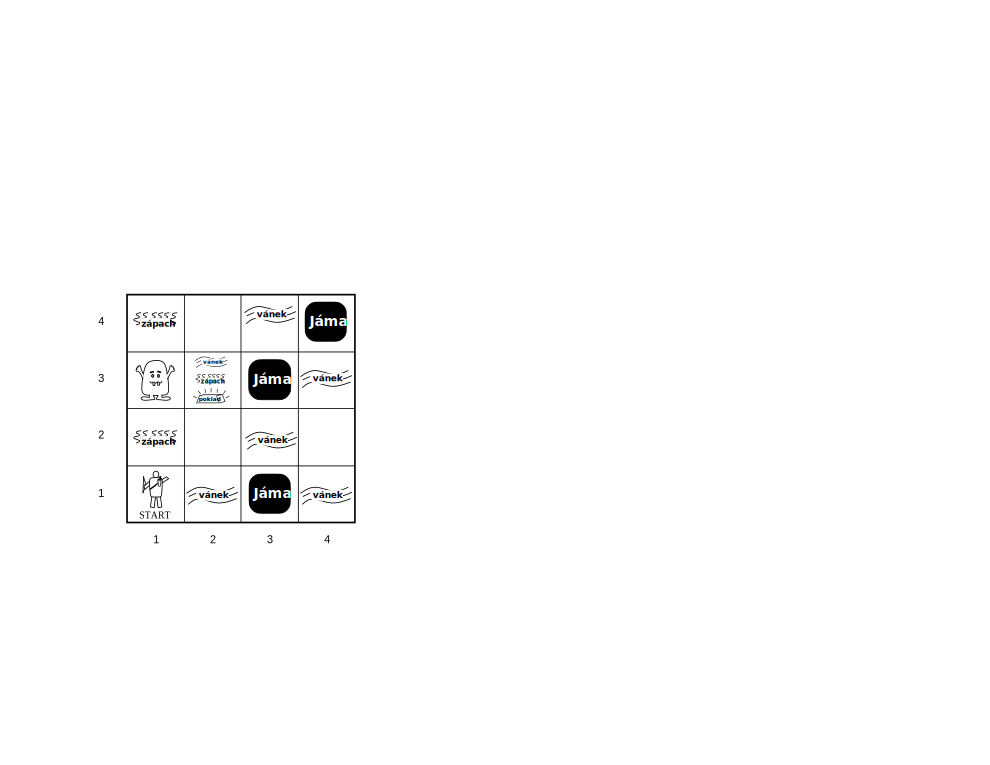
\includegraphics[width=7cm]{wumpus.pdf}
\end{center}
\end{frame}


\begin{frame}\frametitle{Průchod jeskyní}
(1,1) => (2,1) => (1,1) => (1,2) => (2,2) => ... => (2,3) => (2,2) => (1,2) => (1,1)
\end{frame}

\begin{frame}\frametitle{Znalostní báze --- výroková logika}
 Naše znalostní báze (náš model světa) si bude pro každé políčko
 uchovávat informaci o tom, zda
 \begin{itemize}
  \item to tam fouká ($F_{i,j}$)\pause
  \item to tam zapáchá ($Z_{i,j}$)\pause
  \item je tam příšera ($P_{i,j}$)\pause
  \item je tam jáma ($J_{i,j}$)\pause
  \item je tam poklad ($Pk_{i,j}$)\pause
  \item tím políček letěl šíp ($S_{i,j}$)\pause
  \item zda jsem políčko navštívil ($N_{i,j}$)
 \end{itemize}\pause
 Dále si bude pamatovat\pause, zda je příšera mrtvá ($Sk$)\pause, zda jsem vystrelil sip ($S$)\pause\ a zda jsem sebral poklad ($Hura$)\pause.
 Naše znalosti o světě pak můžeme zapsat pomocí axiomů\pause\ (formulí výrokové logiky nad proměnnými $F,Z,P,J,Pk$):\pause
 \begin{itemize}
  \item $P_{i,j}\rightarrow (Z_{i-1,j}\wedge Z_{i+1,j}\wedge Z_{i,j-1}\wedge Z_{i,j+1})$\pause
  \item $J_{i,j}\rightarrow (F_{i-1,j}\wedge F_{i+1,j}\wedge F_{i,j-1}\wedge F_{i,j+1})$\pause
  \item $P_{i,j}\wedge S_{i,j}\rightarrow Sk$
 \end{itemize}
\end{frame}

\begin{frame}[fragile]\frametitle{Agent Hrdina}
\begin{python}
def agentHrdina(akce, vjem):
  if vjem == 'zapach':
    self.baze.update('Z'+self.pos, True)
  ...
  if len(self.plan) > 0:
    return self.plan.pop()
  
  # Pokud jsem nasel poklad tak ho seberu 
  # a vydam se zpet
  if vjem == 'poklad':
    plan = self.route((1,1))
    return 'seber_poklad'
\end{python}
\end{frame}
\begin{frame}[fragile]\frametitle{Agent Hrdina, pokračování $\ldots$}
\begin{python}
  # Zkusim najit prokazatelne bezpecne 
  # nenavstivene policko a vydat se tam
  for pos in jeskyne:
    if self.baze.ask('not J'+pos+' and not P'+pos):
      if self.baze.ask('not N'+pos):
        self.plan = self.route(pos)
        if self.plan:
          return self.plan.pop()
  
  # Pokud jsem jeste nestrilel, tak to zkusim
  if self.baze.ask('not S'):
    return 'vystrel'
\end{python}
\end{frame}
\begin{frame}[fragile]\frametitle{Agent Hrdina, pokračování $\ldots$}
\begin{python}
    
  # Zkusim najit alespon policka, ktera nejsou 
  # prokazatelne nebezpecna a vydat se tam
  for pos in jeskyne:
    if not self.baze.ask(['J'+pos+' or P'+pos]):
      if self.baze.ask('not N'+pos):
        self.plan = self.route(pos)
        if self.plan:
          return self.plan.pop()
  
  # Vzdej to a vylez z jeskyne
  plan = self.route((1,1))
\end{python}
\end{frame}


\begin{frame}\frametitle{{\tt baze.ask}: Sémantické vs Syntaktické odvozování}
Jsou v zásadě dvě možnosti, jak zjišťovat platnost formulí:\pause
\vskip0.5cm
\emph{Ověřování modelů} (model checking)\pause
 \begin{itemize}
 \item procházení všech modelů (enumerace pravdivostní tabulky)\pause
 \item Davis-Putnam-Logemann-Loveland algoritmus (DPLL)\pause
 \item lokální prohledávání (minimalizace konfliktů), WalkSAT\pause
 \end{itemize}
\emph{Dokazování}\pause
 \begin{itemize}
  \item hledání důkazů aplikací odvozovacích pravidel\pause
  \item rezoluce
 \end{itemize}
\end{frame}

\begin{frame}[fragile]\frametitle{Sémantické odvozování --- enumerace}
\begin{python}
def enumSAT( clauses, unassigned_vars, partial_model):
    if len(unassigned_vars) == 0:
        return sat(clauses, partial_model) == 'yes'
    else:
        var = unassigned_vars.pop()
        partial_model[var] = True
        if enumSAT( clauses, unassigned_vars, partial_model): return partial_model
        partial_model[var] = False
        if enumSAT( clauses, unassigned_vars, partial_model): return partial_model
        unassigned_vars.append(var)
        del partial_model[var]
\end{python}
\end{frame}

\begin{frame}[fragile]\frametitle{Sémantické odvozování --- DPLL}
\begin{python}
def dpll(clauses,unassigned_vars,partial_model):
  status = SAT(clauses, partial_model)
  
  # Pokud castecny model splnuje vsechny formule
  # mame vyhrano
  if status == 'all_sat'
    return partial_model
  
  # Pokud castecny model nejakou formuli 
  # nesplnuje, muzeme ho rovnou zahodit
  elif status == 'some_fail':
    return None
\end{python}
\end{frame}
\begin{frame}[fragile]\frametitle{DPLL, pokračování $\ldots$}
\begin{python}    
  # Pokud je nejaka promenna ryzi, vim, 
  # jakou musi mit hodnotu
  var,val = extract_pure( clauses, unassigned_vars )
  if var:
      partial_model[var] = val
      if dpll( clauses, unassigned_vars, partial_model ): return partial_model
      else:
          del partial_model[var]
          unassigned_vars.append(var)
          return None
\end{python}
\end{frame}
\begin{frame}[fragile]\frametitle{DPLL, pokračování $\ldots$}
\begin{python}  
  # Pokud je v nejake klauzuli pouze jedna
  # promenna, vim, jakou musi mit hodnotu
  var, val = extract_unit_var(clauses, unassigned_vars)
  if var:
      partial_model[var] = val
      if dpll( clauses, unassigned_vars, partial_model): return partial_model
      else:
          del partial_model[var]
          unassigned_vars.append(var)
          return None
\end{python}
\end{frame}
\begin{frame}[fragile]\frametitle{DPLL, pokračování $\ldots$}
\begin{python}
  # Zvolme jednu neohodnocenou promennou, ohodnotme ji
  # a zkusme rekurzivne postavit model 
  var = unassigned_vars.pop()
  partial_model[var] = True
  if dpll( clauses, unassigned_vars,partial_model): return partial_model
  partial_model[var] = False
  if dpll( clauses, unassigned_vars,partial_model): return partial_model
  unassigned_vars.append(var)
  del partial_model[var]
  return None
\end{python}

\end{frame}

\begin{frame}[fragile]\frametitle{Sémantické odvozování --- WalkSAT}
\begin{python}
def walkSAT(clauses, p, maxflips):
  vars  = extract_vars(klauzule)
  model = random_assignment(vars,[True,False])

  # Zkousej prehazovat promenne 
  while maxflips > 0:
    maxflip -= 1
    
    # Pokud model splnuje klauzule, vyhrali jsme
    if sat(model, clauses): return model
    
    # Zvol si nahodnou klauzuli
    clause = random.choose(clauses)
    cvars = extract_vars(clause)
\end{python}
\end{frame}
\begin{frame}[fragile]\frametitle{WalkSAT, pokračování $\ldots$}
\begin{python}
    if rand.random() < p:
      # S pravdepodobnosti p prehod nahodne
      # zvolenou promennou
      var = random.choose(cvars)
      model[var] = not model[var]
    else:
      # Prehod promennou, ktera maximalizuje
      # pocet splnenych formuli
      max_sat = 0
      vmax = cvars[0]
      for var in cvars:
        model[var] = not model[var]
        if countSAT(model, clauses) > max_sat:
          vmax = var
          max_sat = countSAT(model,clauses)
        model[var] = not model[var]
      model[vmax] = not model[vmax]        
  return None
\end{python}
\end{frame}

\begin{frame}\frametitle{SAT, Fázový přechod}
\begin{center}
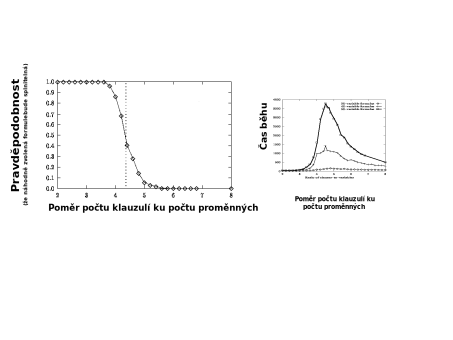
\includegraphics[width=10cm]{sat-phase-transition.pdf}
\vskip2cm
\tiny
(Zdroj: \url{http://www.compphys.uni-oldenburg.de/en/download/talks/pekka_orponen.pdf})
\end{center}

\end{frame}

\begin{frame}\frametitle{Dokazování --- rezoluce}
\begin{block}{}
\begin{center}
Základní krok\pause
\end{center}
\end{block}
\begin{displaymath}
 \frac{a\vee b, -b}{a}
\end{displaymath}\pause
\begin{center}
Obecně\pause
\end{center}
\vskip1cm
\begin{displaymath}
 \frac{x_0\vee\cdots \alt<5->{\alert{x_k}}{x_k}\vee\cdots x_n, y_0\vee\cdots \vee \alt<5->{\alert{y_l}}{y_l}\vee\cdots y_m}
{x_0\vee\cdots\vee \alt<6>{\textcolor{blue}{x_{k-1}\vee x_{k+1}}}{x_{k-1}\vee x_{k+1}}\vee\cdots\vee x_n\vee 
 y_0\vee\cdots \alt<6>{\textcolor{blue}{y_{l-1}\vee y_{l+1}}}{y_{l-1}\vee y_{l+1}}\vee\cdots\vee y_m},
\end{displaymath}
kde 
\begin{displaymath}
 \alt<5->{\alert{x_k}}{x_k} = \alt<5->{\alert{-y_l}}{-y_l}.
\end{displaymath}
\end{frame}

\begin{frame}[fragile]\frametitle{Rezoluce --- algoritmus}
\begin{block}{}
\begin{center}
Algoritmus\pause
\end{center}
\end{block}
\begin{center}
Chceme dokázat $\varphi$ z axiomu $\psi$.\pause
\end{center}
\begin{enumerate}
 \item[1.] Přepiš formuli $\psi\wedge\neg\varphi$ do CNF, seznam klauzulí budiž $K_0=K$.\pause
 \item[2.] Pokud žádné dvě klauzule v $K$ neobsahují komplementární literál, vrať {\tt False}\pause
 \item[3.] Odeber z $K$ dvě klauzule s komplementárním literálem, aplikuj na ně základní krok rezoluce\pause
 \item[4.] Pokud je výsledkem prázdná klauzule, vrať {\tt True}\pause
 \item[5.] Jinak vlož výsledek zpět do K a pokračuj krokem 2
\end{enumerate}

% \begin{enumerate}
%  \item[1.] Přepiš formuli $\psi\wedge\neg\varphi$ do CNF, seznam klauzulí budiž $K_0=K$.\pause
%  \item[2.] Pro každou dvojici klauzují $C_1,C_2$ v $K$ proveď:\pause
%  \begin{itemize}
%   \item[2a] pokud mají $C_1$ a $C_2$ komplementární literál, aplikuj na ně základní krok rezoluce\pause
%   \item[2b] pokud je výsledkem předchozího kroku prázdná klauzule, vrať \emph{True}\pause
%   \item[3c] jinak přidej výsledek do $New$\pause
%  \end{itemize}
%  \item[3.] Pokud je $New\subseteq K$ vrať \emph{False}\pause
%  \item[4.] Polož $K=K\cup New$ a jdi zpět na 2.
% \end{enumerate}

\end{frame}

% \begin{frame}\frametitle{Úplnost rezoluce}
%  \begin{enumerate}
%   \item[1.] Algoritmus vždy skončí\pause, budiž $K_{fin}$ hodnota $K$ na konci.\pause
%   \item[2.] Pokud vrátí false, pak žádné dvě klauzule v $K_{fin}$ neobsahují komplementární literál, tudíž lze 
%             sestrojit model $K_{fin}$.
%   \item[3.] Pokud tento model není modelem $K_0$, existují klauzule $c\in K_0$ a $d\in K_{fin}$ obsahující komplementární
%   \begin{itemize}
%    \item Postupně konstruujeme přiřazení
%   \end{itemize}
% 
%  \end{enumerate}
% 
% \end{frame}



\begin{frame}\frametitle{Dokazování --- Hornovské klauzule}
\emph{Hornovská klauzule} je klauzule tvaru\pause
\begin{displaymath}
 x_0\wedge\cdots \wedge x_n\rightarrow x_{n+1}\pause,
\end{displaymath}
t.j. klauzule, která v obsahuje pouze jeden pozitivní literál ($x_{n+1}$).\pause
\vskip1cm
\emph{Hornovská formule} je formule, jejíž CNF je konjunkce hornovských klauzulí.
\end{frame}

\begin{frame}[fragile]\frametitle{Hornovské klauzule --- dopředné řetězení}
\begin{block}{}
 Chceme zjistit, zda lze ze znalostní báze sestávající z hornovských klauzulí a faktů\pause\ (pozitivních literálů) 
 odvodit fakt $x$.
\end{block}\pause
Algoritmus začne z faktů ze znalostní bázi\pause\ a v každém kroku k nim přidá závěr každé hornovské formule, jejíž premisy už jsou známy.\pause\
Pokud tímto postupem dostane fakt $x$ vrátí \emph{True}\pause\ jinak vrátí \emph{False}.
\end{frame}

\begin{frame}[fragile]\frametitle{Hornovské klauzule --- dopředné řetězení}
\begin{python}
def forwardChaining( baze, x ):
  # Spocti kolik ma kazda klauzule v bazi premis
  count = count_premises(baze.clauses)
  odvozeno = []
  work = baze.facts
  while len(work) > 0:
    fact = work.pop()
    if fact == x: return True
    if fact not in odvozeno:
      odvozeno.append(fact)
      for c in baze.clauses:
        if fact in c.premises:
          count[c] -= 1
          if count[c] == 0:
            work.append(c.conclusion)
  return False
\end{python}
\end{frame}

\begin{frame}[fragile]\frametitle{Hornovské kaluzule --- zpětné řetězení}
\begin{itemize}
 \item Dopředné řetězení vychází z faktů a odvozuje nové, dokud nenarazí na $x$.\pause
 \item Odvodí spoustu zbytečností.\pause
 \item Zpětné odvození odvozuje pouze fakta, která jsou perspektivní, t.j. vedou k $x$.
\end{itemize}
\end{frame}

\begin{frame}[fragile]\frametitle{Hornovské kaluzule --- zpětné řetězení}
\begin{python}
def backwardChaining( baze, x ):
  if x in baze.facts:
    return True
  for c in baze.clauses:
    if x == c.conclusion:
      can_sat_c = True
      for y in c.premises:
        if not backwardChaining( baze, y ):
          can_sat_c = False
          break
      if can_sat_c:
        baze.facts.append(x)
        return True
  return False
\end{python}
\end{frame}
\end{document}